\documentclass[a4paper,fleqn]{cas-sc}
\usepackage{amsmath,amssymb}
\usepackage{booktabs}
\usepackage{graphicx}
\usepackage{hyperref}

\begin{document}

\shorttitle{SAT Encodings for the N-Queens Problem}
\title [mode = title]{SAT Encodings for the N-Queens Problem: A Recovered and Updated Experimental Report}
\author[1]{Assignment 1}
\affiliation[1]{organization={Faculty of Information Technology}, city={Local environment}}

\begin{abstract}
The N-Queens problem is a compact feasibility benchmark in which the choice of
representation strongly affects both formula size and solving time. This report
reconstructs the structure of the supplied reference report while restricting
quantitative claims to experiments actually present in the project. The SAT
model uses one Boolean variable per board cell, row and column exactly-one
constraints, and diagonal at-most-one constraints. Pairwise, Sequential,
Binary, and Commander encodings are available, and Glucose3 and CaDiCaL are
used through PySAT. Binary-cell MIP models are provided for CPLEX MIP and
Gurobi, while CPLEX CP Optimizer uses an integer column model. The historical
SAT experiment contains 80 records through $N=64$; the approved medium matrix
contains 40 correctness records and 87 performance records; and a separate
Gurobi follow-up contains 15 records through $N=8$, with an existing validated
$N=16$ artifact. OR-Tools is recorded as unavailable. Results distinguish
SAT, UNSAT, FEASIBLE, TIMEOUT, ERROR, and license-limit outcomes, and every
reported solution is checked by an independent validator.
\end{abstract}

\maketitle

\section{Introduction}

\subsection{Context and problem scope}
The N-Queens problem asks for a placement of $n$ queens on an $n\times n$
board such that no two queens share a row, column, or diagonal. The present
assignment concerns the ordinary feasibility problem on an initially empty
board: one valid placement is sufficient for a satisfiable instance, whereas
an unsatisfiable result must be established by the selected exact solver.

N-Queens is useful for comparing exact solving paradigms because the same
combinatorial object can be represented in several ways. A SAT model expands
conflicts into clauses; a constraint-programming model uses finite-domain
variables and global constraints; and an integer-linear model uses binary cell
variables and linear inequalities. These representations expose different
construction costs and propagation mechanisms, so a smaller formula is not
automatically a faster experiment.

\subsection{Assignment requirements and project scope}
The assignment requires an implemented solver for the selected logic-puzzle
topic, an experimental comparison with exact methods such as ILP and CP, and a
scientific-paper-style report using the Elsevier \texttt{cas-sc} template. It
explicitly names CPLEX CP, CPLEX MIP, Gurobi, and CP-SAT as comparison targets
and encourages alternative AMO/ALO encodings such as Binary, Commander,
Product, and Sequential Counter.

The current project implements the required SAT solver and the Pairwise and
Sequential encodings, and extends the comparison with Binary and Commander.
It also contains adapters for CPLEX MIP, CPLEX CP Optimizer, Gurobi, and
OR-Tools CP-SAT. The first three non-SAT backends have usable measurements in
the available environment. OR-Tools is not installed and no result is
claimed for it. Recursive 2-Product, integer-column MIP, and a constructive
algorithm are outside the implemented scope of this submission.

\subsection{Contributions of this report}
The report makes four project-specific contributions:

\begin{enumerate}
  \item a common N-Queens formulation with four implemented SAT AMO encodings;
  \item independent validation of decoded placements and explicit solver
        status preservation;
  \item separate historical, medium-matrix, and Gurobi follow-up artifacts;
  \item an empirical discussion that separates model construction, solver
        time, total wall time, formula size, and environmental limitations.
\end{enumerate}

\section{Problem Definition and Baseline Formulations}

Let $I_n=\{0,\ldots,n-1\}$ index rows and columns. A placement can be
represented by a vector $Q=(q_0,\ldots,q_{n-1})$, where $q_i$ is the column
occupied in row $i$. The constraints are
\begin{align}
  0\le q_i<n &\quad (i\in I_n),\\
  \operatorname{AllDifferent}(q_0,\ldots,q_{n-1}) & ,\\
  \operatorname{AllDifferent}(q_0+0,\ldots,q_{n-1}+n-1) & ,\\
  \operatorname{AllDifferent}(q_0-0,\ldots,q_{n-1}-(n-1)) & .
\end{align}
The second condition prevents shared columns, and the last two prevent shared
anti-diagonals and main diagonals respectively.

\subsection{Constraint-programming model}
The CPLEX CP Optimizer adapter uses one integer variable $q_i\in[0,n-1]$
per row, an \texttt{AllDifferent} constraint on columns, and pairwise diagonal
inequalities. This is a compact representation: exactly one queen per row is
implicit in the variable vector. The adapter reports \texttt{FEASIBLE} when a
validated placement is returned; it does not relabel feasibility as
\texttt{OPTIMAL}.

\subsection{Binary-cell ILP model}
For MIP solvers, let $X_{i,j}\in\{0,1\}$ indicate a queen at cell $(i,j)$.
The implemented model contains
\begin{align}
  \sum_{j=0}^{n-1}X_{i,j}&=1 && (i\in I_n),\\
  \sum_{i=0}^{n-1}X_{i,j}&=1 && (j\in I_n),\\
  X_{i,j}+X_{i',j'}&\le 1 && (i-i'=j-j',\ i\ne i'),\\
  X_{i,j}+X_{i',j'}&\le 1 && (i-i'=-(j-j'),\ i\ne i').
\end{align}
The CPLEX MIP and Gurobi adapters use this binary-cell representation. A
returned placement is decoded row by row and checked independently. The
Community Edition of CPLEX limits the larger MIP instance; this is an
environmental restriction, not evidence that the MIP formulation is
unsatisfiable.

\section{SAT Methodology}

\subsection{Common board variables and constraints}
The SAT variable $B_{i,j}$ has a positive integer identifier for board cell
$(i,j)$. Each row and column receives an at-least-one clause and an at-most-one
constraint. Every non-singleton main diagonal ($i-j$ constant) and
anti-diagonal ($i+j$ constant) receives an at-most-one constraint. No
at-least-one clause is needed for a diagonal: the row and column constraints
already require exactly $n$ selected cells.

For a group $G=(x_0,\ldots,x_{m-1})$, the AMO condition is
\[
  \operatorname{AMO}(G)=\bigwedge_{0\le a<b<m}(\lnot x_a\lor\lnot x_b)
\]
for the Pairwise case. The other encodings introduce auxiliary variables but
preserve the projection property
\[
  \operatorname{AMO}(G)\quad\Longleftrightarrow\quad
  \exists Y\ E(G,Y),
\]
where $Y$ is the set of auxiliary variables.

\subsection{Pairwise (Binomial) encoding}
Pairwise encoding emits one binary exclusion clause for every pair of inputs.
It has no auxiliary variables and has quadratic cost for one AMO group:
\[
  a_{\rm pw}(m)=0,\qquad c_{\rm pw}(m)=\binom m2.
\]
Its advantage is simplicity and direct propagation. Its disadvantage is the
cubic growth of the complete board's clause count because many groups have
length $n$.

\subsection{Binary encoding}
Binary encoding assigns each input a distinct binary index represented by
$\lceil\log_2m\rceil$ fresh variables. For each input and each index bit, an
implication clause links the input to the corresponding bit value. Two true
inputs would require two different indices and therefore conflict on a bit.
The unused binary codes are harmless because the construction only requires
distinct codes for true inputs. The project handles groups of size zero or one
without auxiliary variables.

The asymptotic auxiliary cost per group is $\Theta(m\log m)$ and the complete
board representation has $\Theta(n^2\log n)$ clauses under this construction.
The exact emitted counts, rather than asymptotic expressions, are used in the
benchmark artifacts.

\subsection{Sequential Counter encoding}
The Sequential encoding introduces a prefix chain. For a group of length
$m\ge2$, it uses $m-1$ auxiliary variables that represent prefix occupancy.
Linking clauses propagate an occupied prefix and forbid a second true input.
Thus both auxiliary variables and clauses are linear in the group size, and
the complete board has quadratic asymptotic growth.

\subsection{Commander encoding}
Commander encoding partitions an input group into consecutive groups of three.
Each non-base group receives a commander variable linked in both directions to
the disjunction of its inputs; the commanders are then encoded recursively.
Groups of size at most three use Pairwise clauses as the base case. This
hierarchy has logarithmic recursion depth and quadratic asymptotic growth for
the complete board under the implemented group size.

\subsection{Scope boundary: recursive Product encoding}
The supplied reference report also describes a recursive 2-Product encoding
and reports large-instance results for it. That encoding is not present in the
current project and was explicitly excluded from the approved implementation
scope. Its original numerical results are therefore not reused as current
project measurements.

\subsection{Formula-size verification}
The current implementation's emitted formula sizes at $n=4$ are shown below.
They are read from the medium correctness/performance artifacts, not copied
from the reference report.

\begin{table}[ht]
\centering
\caption{Observed SAT formula sizes at $n=4$ in the current implementation.}
\label{tab:formula-size}
\begin{tabular}{lrr}
\toprule
Encoding & Variables & Clauses\\
\midrule
Pairwise & 16 & 84\\
Sequential & 40 & 100\\
Binary & 32 & 100\\
Commander & 32 & 116\\
\bottomrule
\end{tabular}
\end{table}

\begin{figure}[ht]
\centering
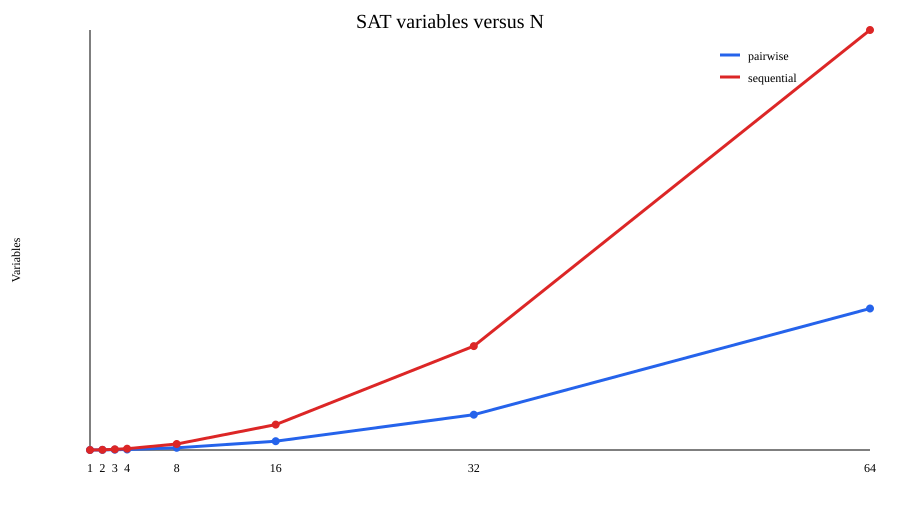
\includegraphics[width=0.85\linewidth]{../results/figures/variables_vs_n.svg}
\caption{Historical SAT variable counts by encoding and board size.}
\label{fig:historical-variables}
\end{figure}

\begin{figure}[ht]
\centering
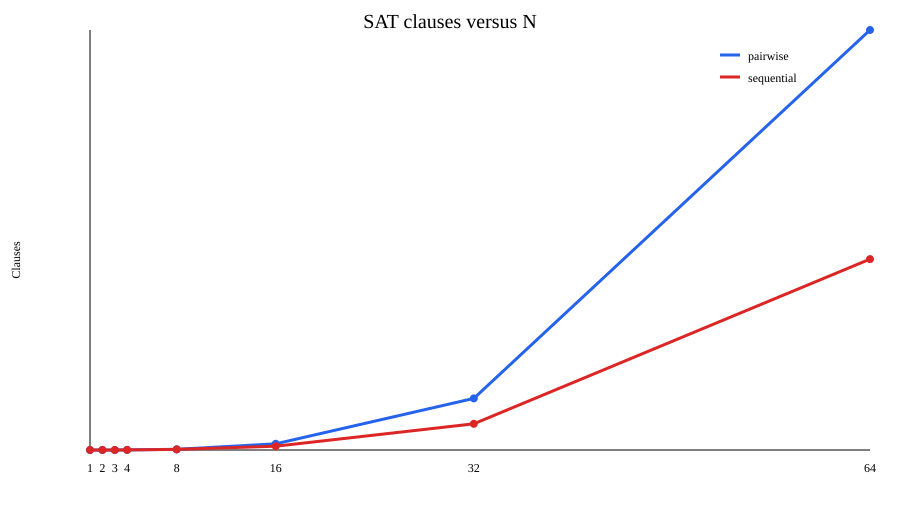
\includegraphics[width=0.85\linewidth]{../results/figures/clauses_vs_n.svg}
\caption{Historical SAT clause counts by encoding and board size.}
\label{fig:historical-clauses}
\end{figure}

\begin{figure}[ht]
\centering
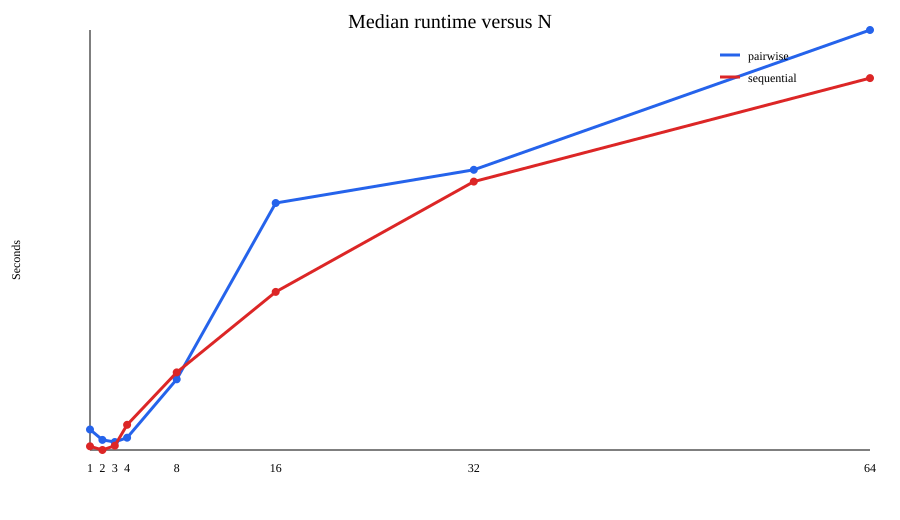
\includegraphics[width=0.85\linewidth]{../results/figures/runtime_vs_n.svg}
\caption{Historical SAT median runtime by encoding and board size.}
\label{fig:historical-runtime}
\end{figure}

\section{Correctness and Independent Validation}

Correctness is separated from performance. The correctness matrix covers
$n\in\{1,2,3,4\}$, including satisfiable and unsatisfiable instances. It
contains four encodings for each of Glucose3 and CaDiCaL, plus CPLEX MIP and
CPLEX CP Optimizer. It contains 40 records in total: 18 SAT, 20 UNSAT, and 2
FEASIBLE, with no timeout or error.

For every backend, a decoded solution is checked by the independent
\texttt{validate\_solution} routine. The validator checks one column per row,
column uniqueness, and both diagonal conditions. A non-null solver model is
not by itself treated as validation success. Unsatisfiable outcomes have no
solution and are not classified as invalid SAT solutions.

The project test suite contains 25 passing tests in the latest recorded run.
It covers known SAT/UNSAT instances, encoding equivalence, formula sizes,
invalid inputs, timeout handling, optional dependency behavior, historical
JSON/CSV schema, CPLEX adapters, and the Gurobi adapter.

\section{Experiments and Results}

\subsection{Experimental setup}
The project retains three distinct experimental families:

\begin{enumerate}
  \item the historical SAT benchmark, with $n=1,2,3,4,8,16,32,64$, two
        encodings, and five trials per configuration;
  \item the approved medium matrix, with a 10-second timeout and three trials
        for performance cells at $n=4,8,16$;
  \item the Gurobi follow-up, with a 10-second timeout, three trials, and
        $n=1,2,3,4,8$; the existing $n=16$ Gurobi artifact is kept separate.
\end{enumerate}

For each comparison record, the schema stores the instance, method, backend,
encoding, trial, timeout, solver version, model-size fields, normalized
status, raw backend status, validation flag, error, build time, solve time,
and total wall time. Total wall time includes the adapter call. Build and
solver times are recorded separately, but their exact coverage differs by
backend: SAT build time is CNF construction, while the mathematical-model
adapters measure model construction after dependency import. This difference
is reported as a limitation rather than hidden.

\subsection{Historical SAT benchmark}
The historical artifact contains 80 records: eight board sizes, two SAT
encodings, and five repetitions for each cell. The status distribution is 60
SAT and 20 UNSAT, with no timeout or error. The corresponding JSON and CSV
files agree, and their summary medians are computed from the raw completed
records.

\subsection{Medium encoding and backend matrix}
The performance matrix contains 87 records. Glucose3 and CaDiCaL each cover
four encodings at $n=4,8,16$, giving 72 records. CPLEX CP Optimizer contributes
nine records at the same three sizes. CPLEX MIP contributes six records at
$n=4,8$; $n=16$ is deliberately omitted after the Community Edition model
limit was verified. The distribution is 78 SAT and 9 FEASIBLE, with no
timeout, error, or license-limit record in this pre-filtered matrix.

\begin{table}[ht]
\centering
\caption{Median total time for selected current medium-matrix cells.}
\label{tab:medium-runtime}
\begin{tabular}{lrrr}
\toprule
Configuration & $n=4$ & $n=8$ & $n=16$\\
\midrule
Glucose3 + Pairwise & 0.000365 & 0.000823 & 0.018973\\
Glucose3 + Sequential & 0.000309 & 0.000897 & 0.003935\\
Glucose3 + Binary & 0.000334 & 0.000792 & 0.006012\\
Glucose3 + Commander & 0.000310 & 0.000710 & --\\
CPLEX CP Optimizer & 0.029908 & 0.030010 & 0.036320\\
\bottomrule
\end{tabular}
\end{table}

The values in Table~\ref{tab:medium-runtime} are medians from the raw
performance records and are rounded only for display. The complete values,
including build and solver-time medians, remain available in
\texttt{benchmark\_medium\_performance\_summary.json}. The plot below is
generated from that summary.

\begin{figure}[ht]
\centering
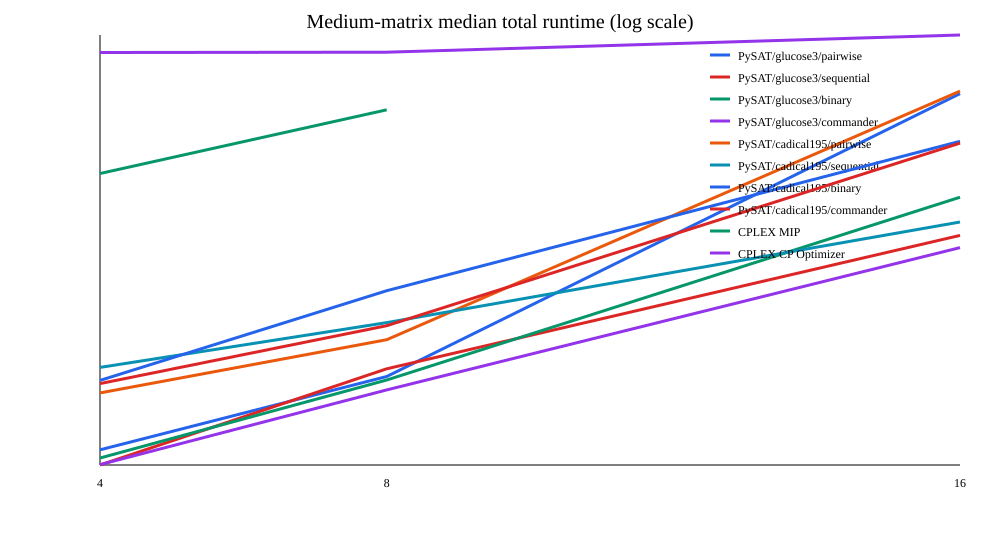
\includegraphics[width=0.9\linewidth]{../results/figures/medium/runtime_by_method.svg}
\caption{Median total runtime for the current medium performance matrix.}
\label{fig:medium-runtime}
\end{figure}

\begin{figure}[ht]
\centering
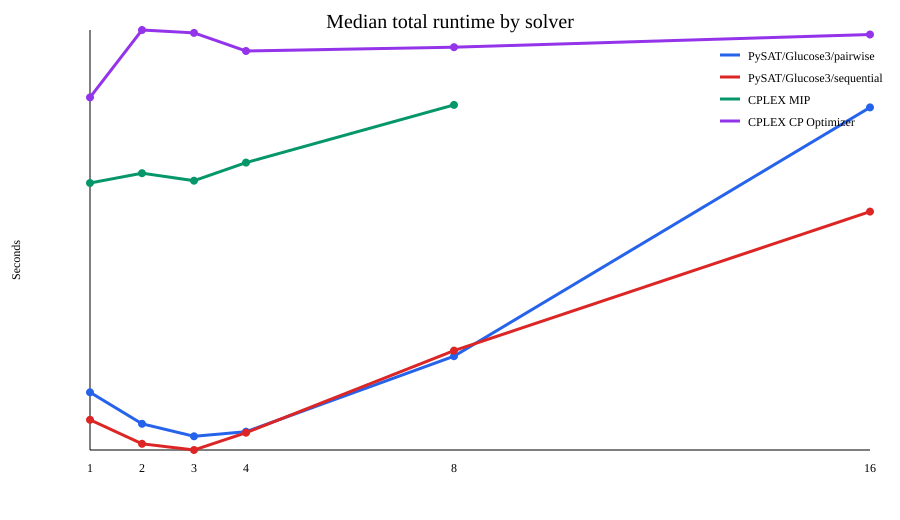
\includegraphics[width=0.85\linewidth]{../results/figures/comparison/runtime_by_solver.svg}
\caption{Median runtime by solver and encoding in the original comparison artifact.}
\label{fig:comparison-runtime}
\end{figure}

\begin{figure}[ht]
\centering
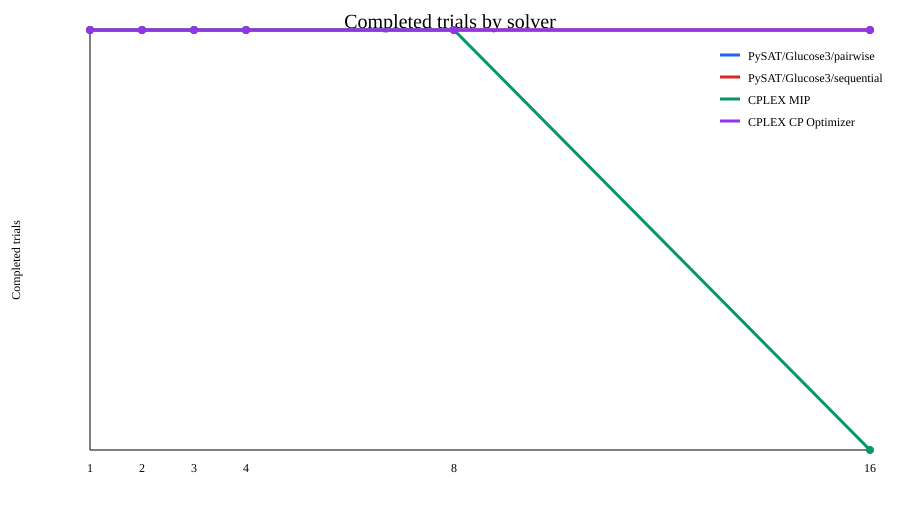
\includegraphics[width=0.85\linewidth]{../results/figures/comparison/completed_by_solver.svg}
\caption{Completed trials by solver and size in the original comparison artifact.}
\label{fig:comparison-completed}
\end{figure}

\subsection{Gurobi follow-up}
The existing Gurobi $n=16$ artifact contains three FEASIBLE records, each with
\texttt{solution\_valid=true}. The follow-up artifact contains 15 records for
$n=1,2,3,4,8$: 9 FEASIBLE records and 6 UNSAT records, with no timeout or
error. Gurobi 13.0.3 is recorded in its metadata. A FEASIBLE status means that
Gurobi found a valid placement; it is not renamed OPTIMAL because this is a
feasibility problem without an optimization objective.

\begin{table}[ht]
\centering
\caption{Gurobi follow-up status counts by board size.}
\label{tab:gurobi-followup}
\begin{tabular}{lrrr}
\toprule
$n$ & Trials & FEASIBLE & UNSAT\\
\midrule
1 & 3 & 3 & 0\\
2 & 3 & 0 & 3\\
3 & 3 & 0 & 3\\
4 & 3 & 3 & 0\\
8 & 3 & 3 & 0\\
\bottomrule
\end{tabular}
\end{table}

The Gurobi follow-up is not silently merged with the historical 72-record
comparison or the 87-record medium matrix. It uses the same broad schema and
timeout policy, but its size set and execution time are a separate experiment.

\section{Discussion and Limitations}

The results support encoding- and backend-specific observations, not a
universal ranking. Sequential and Commander reduce the growth of the
Pairwise-style AMO clause family, while Binary uses index bits and a different
propagation structure. The measured runtime depends on both the resulting
formula and the backend. Therefore formula size, construction cost, solver
time, and total wall time should be reported together.

The CPLEX Community Edition limit prevents a fair CPLEX MIP run at $n=16$ in
the medium matrix. Gurobi is available in the current environment, but the
follow-up covers only five sizes plus a separate $n=16$ artifact. OR-Tools is
not installed, so no CP-SAT performance conclusion is possible. The supplied
reference report discusses five encodings and runs up to $n=1331$; those
large-scale Product and CP-SAT results are not current project measurements
and are intentionally not reproduced as if they were.

The experiments use one local environment and a small number of repetitions.
Backend startup and dependency-import behavior affect the measured intervals.
The current figures use SVG files, so compilation requires a LaTeX setup that
supports SVG or a prior conversion to PDF/PNG. No PDF compilation is claimed
in the current environment because no LaTeX compiler or \texttt{cas-sc.cls}
was available.

\section{Conclusion}

The project provides a validated SAT N-Queens implementation with four AMO
encodings, two PySAT backends, CPLEX MIP, CPLEX CP Optimizer, and Gurobi
adapters. The historical and medium artifacts establish correctness and
repeatable small-to-medium measurements. The Gurobi follow-up confirms valid
solutions and UNSAT outcomes on its stated sizes, while preserving the
distinction between FEASIBLE, UNSAT, and unavailable or license-limited
outcomes.

The evidence supports selecting an encoding together with a backend rather
than selecting solely by the number of variables or clauses. Larger-scale
claims from the supplied reference report require implementation and
measurement of the missing Product and CP-SAT configurations before they can
be attributed to this project.

\section*{Data Availability}
The source repository is available at
\url{https://github.com/DunnTapCodee/N-Queens-Solver}. The repository contains
source code, tests, benchmark JSON/CSV files, summaries, backend manifest,
figures, and the report source. Historical files are preserved separately from
the medium and Gurobi follow-up artifacts.

\begin{thebibliography}{00}
\bibitem{gent} I. P. Gent, C. Jefferson, and P. Nightingale, ``Complexity of
N-Queens Completion,'' IJCAI, 2018.
\bibitem{ortools} Google OR-Tools, ``The N-queens Problem,'' official
documentation. No OR-Tools result is claimed in this project because the
package is unavailable.
\bibitem{sinz} C. Sinz, ``Towards an Optimal CNF Encoding of Boolean
Cardinality Constraints,'' CP, 2005.
\bibitem{klieber} W. Klieber and G. Kwon, ``Efficient CNF Encoding for
Selecting 1 from N Objects,'' 2007.
\bibitem{chen} J. Chen, ``A New SAT Encoding of the At-Most-One Constraint,''
2010.
\bibitem{pysat} A. Ignatiev et al., ``PySAT: A Python toolkit for prototyping
with SAT oracles,'' SAT, 2018.
\end{thebibliography}

\end{document}
